\section{An\'alisis del M\'etodo Moreno-Dominguez}

Utilizar \textit{Hierarchical Agglomerative Clustering} con la distancia 
coseno y el \textit{linkage} centroide presenta al menos dos desventajas. 
Primero, la distancia coseno obliga a tener que comparar expl\'icitamente cada
centroide con los clusters existentes. Notemos que esto implica mantener los
clusters en memoria. Por otro lado, el promedio de probabilidades no
necesariamente representa una probabilidad \cite{Pohl2007}. Esto quiere decir
que el centroide de un grupo de tractogramas no necesariamente representa un
tractograma. \\

\subsection{Clustering de vectores colineales}

\begin{figure}[h!]
        \centering
        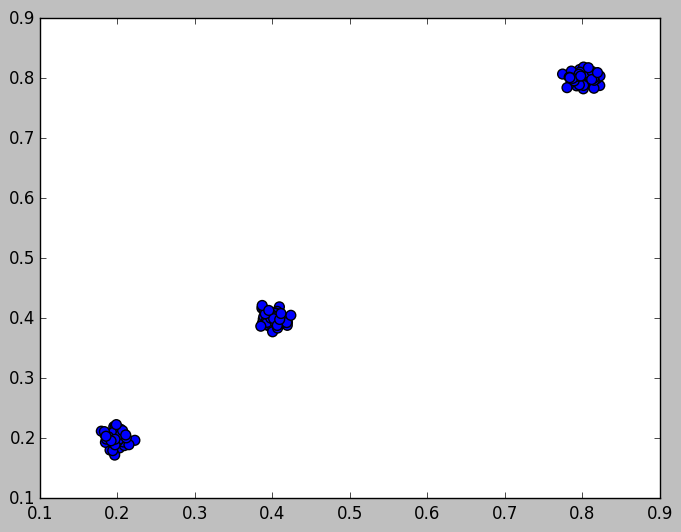
\includegraphics[width=0.5\textwidth]{img/3pop.png}
        \caption{Tres cluster colineales\-}
        \label{fig:3clusters}
\end{figure}

La distancia coseno es una forma de medir co\-rrelaci\'on entre vectores. Por ello,
cuando lo que se intenta agrupar son vectores colineales el resultado es aleatorio.
Por ejemplo, cuando se aplica el procedimiento sobre los puntos de la Figura
\ref{fig:3clusters} el resultado del clustering es la Figura \ref{fig:3moreno}.
Usando LogOdds y la m\'etrica euclidiana se consigue el \textit{clustering} de 
la Figura \ref{fig:3logit}.\\

\begin{figure}[h!]

\centering                                                                                                          
\begin{minipage}[b]{0.85\textwidth}
    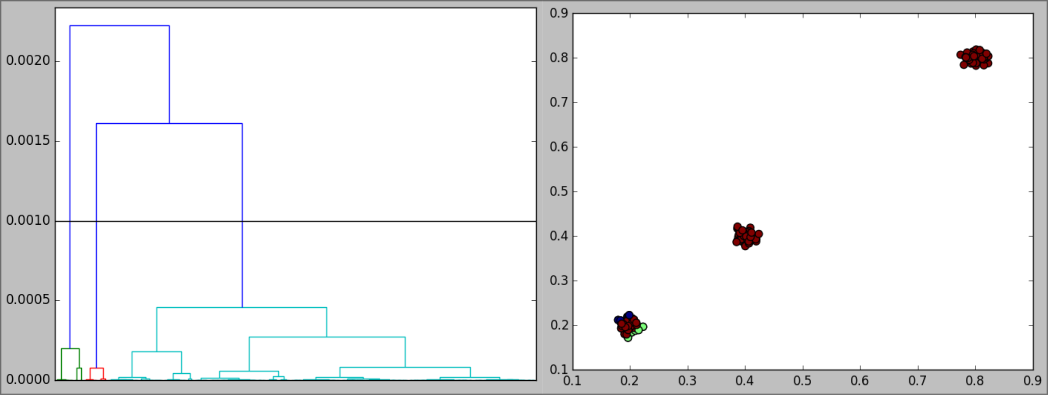
\includegraphics[width=\textwidth]{img/3pop_moreno.png}
    \caption{Clustering resultado de utilizar el m\'etodo Moreno}
    \label{fig:3moreno}
\end{minipage} ~

\end{figure}  

Los tractogramas son im\'agenes que por su naturaleza tienen muchos voxels con 
valores peque\~nos. La Figura \ref{fig:hist_tract} muestra el histograma de los
valores en los tractogramas del \'Area de Broca. Esta gran cantidad
de voxels con valores tan bajos podr\'ia generar ruido en las correlaciones.  

\begin{figure}[h!]
              \centering                                                                                                          
\begin{minipage}[b]{0.8\textwidth}
    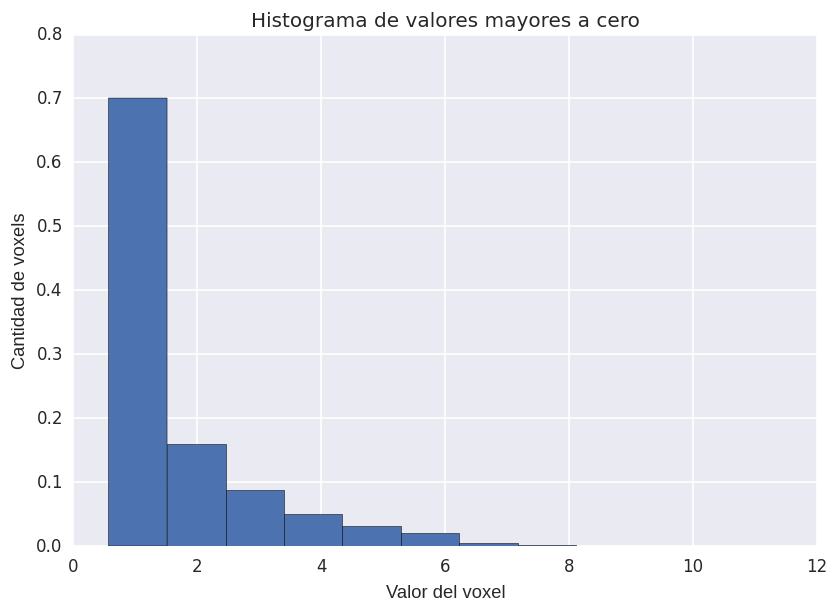
\includegraphics[width=\textwidth]{img/hist_tract.png}
    \caption{Histograma normalizado de los valores en los tractogramas del \'Area de Broca}
    \label{fig:hist_tract}
\end{minipage} ~

\end{figure}  


\subsection{Relaci\'on m\'etrica-\textit{linkage}}

La Figura \ref{fig:cos_cen} muestra cuatro vectores, sus posiciones en coordenadas
polares son: $ p_1 = (0.4, 45^\circ)$;  $p_2 = (0.3, 25^\circ)$;  $p_3 = (0.4, 66^\circ)$
y $p_4 = (0.4, 4.5^\circ) $ \\

Podemos apreciar que al principio $d(p_2,p_3) < d(p_3,p_4) < d(p_1,p_2)$, siendo
$d(x,y)$ la distancia coseno. Sin embargo, luego de utilizar el 
\textit{linkage centroid} sucede que $d(p_1,p_c) < d(p_4,p_c)$. $p_4$
es ahora el punto que mas lejos est\'a del centroide. Creando un representante
$p_m$ usando el \'angulo medio entre $p_2$ y $p_3$ esto no sucede. Este fen\'omeno
se da porque la distancia coseno tiene en cuenta el \'angulo pero el centroide
no. Por lo tanto el centroide no caracteriza al punto medio respecto a la
distancia coseno.\\

\begin{figure}[h!]
                                                                                                                        
\begin{minipage}[b]{\textwidth}
    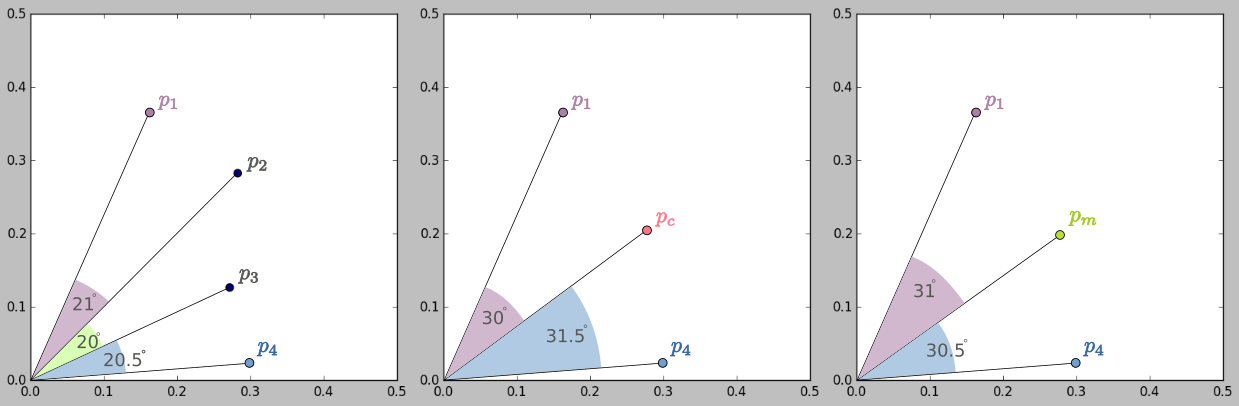
\includegraphics[width=\textwidth]{img/cosine_centroid.png}
    \caption{El centroide no representa el punto medio respecto al \'angulo}
    \label{fig:cos_cen}
\end{minipage} ~

\end{figure}  

\subsection{Complejidad algor\'itmica del Clustering}

En todo el proceso el paso mas caro en t\'erminos computacionales es el
\textit{clustering}. En cada iteraci\'on del algoritmo es necesario comparar 
expl\'icitamente cada nuevo centroide con todo el resto de los clusters. Esto 
es costoso computacionalmente. Por cada iteraci\'on es necesario hacer $O(c^2 m)$
operaciones para recalcular todas las distancias, donde $c$ es la cantidad de
clusters y $m$ es la longitud de los mismos. Dadas $n$ semillas iniciales, la 
cantidad de iteraciones a realizar son $n-1$. La complejidad de este m\'etodo es
$O(n^3 m)$.

